\chapter{Outcome and Measurements}

In this chapter the outcome is measured and evaluated.

%\todo{compare to initial deliverable requirements?}

\section{What did not work as expected}

It is impossible to plan a system ahead of time without making some mistakes.
The biggest issue that surfaced on an early implementation of Winslow was caused by too short-termed EXTEND signals (see \autoref{message:extend}).
In combination with short but high network bandwidth usages, the event was published too late, which led the other instances consider the node to have failed.
This was solved by increasing lock timeouts and issuing the EXTEND signal halfway through the timeout instead of very close to the end.
%\todo{timeout for events might be reached when in between the bandwidth is used by a copy of a large file and the extend signal is because of that deferred, stages that are fine are then marked as failed}

%\todo{. old sections}

\section{User Authentication and Security}
\label{outcome:ssl}

One aspect that was not yet mentioned at all is user authentication and security.
Winslow is prepared in this regards because every project has an owner field and a member list and every web access checks these.
An internal user repository also associates users with groups and provides defaults, such as the user and group \enquote{anonymous} and \enquote{root} for no and full access privileges, respectively.
But at the moment, there is no user login.
Instead, to the system all requests seem to be issued by \enquote{root}.
In the future it is planned to be replaced this by an Single Sign-On implementation that uses the user accounts of our company.
Winslow is then given a user name which it will use to identify the corresponding internal user.
Unknown users are not allowed to see or alter anything, known users will be able to create and view their own projects and projects they are listed as members in.
%\todo{mostly planned, implemented not tested}

Winslow also supports secure HTTP (HTTPS) whenever a SSL certificate is provided\footnote{This can be seen in \autoref{appendix:winslow_installation}}.

\begin{comment}
\section{Storage}

One of the central concerns is the storage management.
The program needs to make input files available on each execution node and collect the results once the computation is complete.
There are a few main architectural strategies to approach this.
Simplified, either at a centralized location which is accessed by all execution nodes, a copy of the input files to the execution nodes or decentralized and distributed between all execution nodes and replication.
The advantages and disadvantages can depend on the specific implementation and is therefore discussed in combination of such (see \autoref{state_of_the_art}).

Further testing is required to decide whether a more complex storage system is required, or the simplicity of a centralized solution outweighs the setup and maintenance overhead.

%\subsection{Hadoop File System}
%\cite{hdfs:main}
%\cite{hdfs:doc}
%\todo{redudancy for evenly distributed}

%\subsection{NFS}
%
%local/per node cache?

\section{Coordination}

Another important concern is the coordination of the nodes.
A central coordinator with external server nodes, such as GitLab and Jenkins have, might not be sufficient for more complex and longer lasting pipelines.
The probability that the master would need to be offline while there is a stage executed, is in the scenario of the desired workflow higher than for GitLab or Jenkins, because the stage is being execution for hours or days.
Coupling stage execution plans on node availability ahead of time, as well as recovering from a sudden master failure implies additional implementation complexity.
A decentralized coordination needs to be able to do this as well, but also allows the usage of the system while a node failed or is unreachable due to maintenance.
With further prototyping and research a reasonable solution shall be found.

\section{Binary distribution}

In a time where containers are common and have proven to be usable, the installation of the binaries directly on the operating system they are executed on shall be avoided.
There shall be no manual, nor automatic but custom file copies of the binaries or images from one server to the other.
Experience shows, that without a proper management, this can easily become a mess, in which it is no longer clear, which files or images belong to which version.
At the same time, making all binaries publicly available through the Docker Hub\cite{docker:hub} is no option either.
Whether a self hosted Docker Registry\cite{docker:registry} could be the solution to this will be determined in further testing.

\section{User Interface}

Providing a useful user interface might not be important to the functionality of the system itself but for the user experience.
A bad user experience will cause a system not to be used.
It became common practice for a rich user experience to be web based and interactive with JavaScript.
For a potentially decentralized system, it is also advantageous to be able to access a disconnected node in the same manner as the remaining system, which further encourages a web based solution.
Web based solutions such as React and Angular shall therefore be investigated for being used as user interface.

\section{Requirements}

\todo{more than first defined - as expected}

\todo{lots more UI shortcuts found necessary while starting to use winslow}

\section{Architecture}

\todo{loosely coupled backend driver}\autoref{architecture:detailed}
\end{comment}



%\section{Internal Locking API}
%\todo{omit? but it plays so well with try with resource: try(var lock = bus.lock(path)) { ..  }}

\section{High Level System Overview}

\autoref{architecture:high-level} shows the high level system overview of Winslow as it is implemented and in use by the end of this thesis in our company.

\begin{figure}[H]
	\centering
	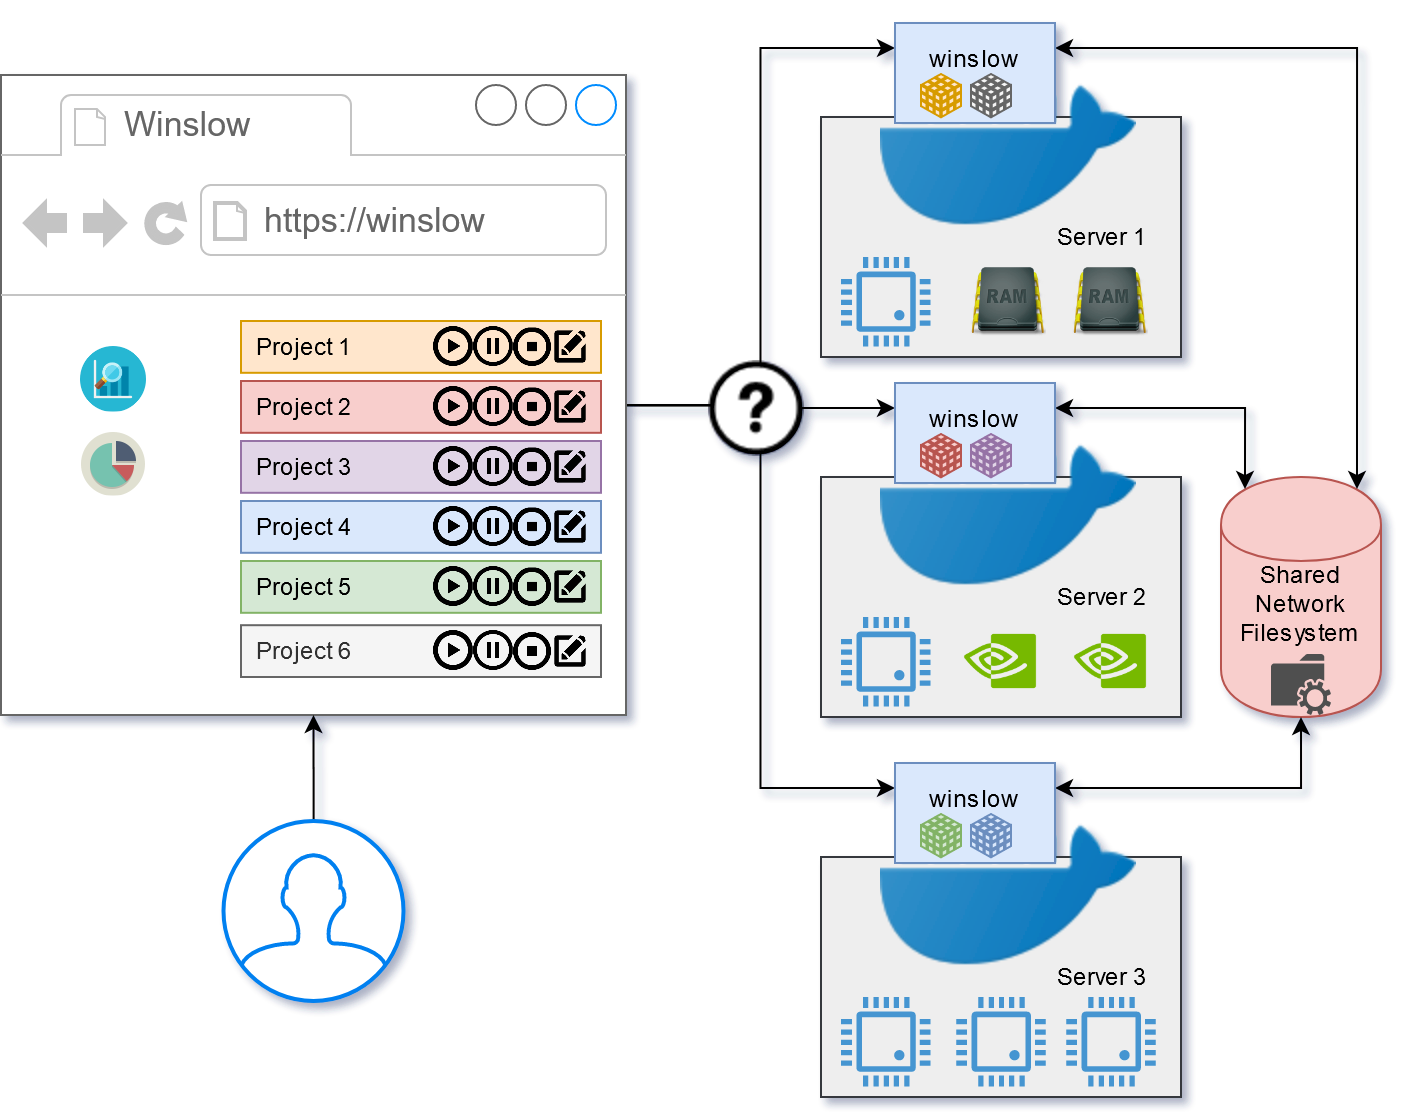
\includegraphics[width=0.8\textwidth]{architecture.png}
	\caption{High level view on the system structure}
	\label{architecture:high-level}
\end{figure}

The user can access the system through the Web-Application, which has no indicating to tell from which Winslow instance it is served.
The three compute nodes supply different hardware, one with 128 GiB RAM, one with 4 NVIDIA RTX 2080 Ti, and one with 32 Intel CPU cores.
All instances access the same NFS share for synchronization and work distribution.


%\todo{explain what is going on in \autoref{architecture:high-level}}

\section{Failure resilience}

One of the requirements for Winslow is to be resilient against node failures.
Node failures can be simulated easily by killing the Docker container of a Winslow instance.
The behaviour that is then displayed depends on whether that killed instance was actually executing a stage.
If it did not, the only change is that in the Web-Application the node with its utilization reports will vanish.

But if it did execute a stage, it held locks for it.
These locks will expire, and after the additional grace period (see \autoref{message:grace_period}), the other instances will notice this, lock the affected project themselves and mark the execution as failed.
Currently, the project is then paused and a user confirmation awaited.
An alternative to this could be to re-schedule the stage automatically.
